\section{Clickstream data: Interface paticipants time-to-action and response to limited budget}
Time-to-action is a widely used metric in decision sciences, where longer decision time often indicates more complex and deeper cognitive processing~\cite{payneAdaptiveDecisionMaker1993}.

\subsection{Time per option}
Our initial analysis examines the time participants spent per option across four experimental conditions. Using the QS system log, we aggregated the total time participants spent per option. For participants in the two-phase interface conditions, this included both organization and voting times. The results are visualized in Figure~\ref{fig:total_time}.

Overall, participants spent slightly more time per option in the two-phase interface than in the text interface. To quantify these observations, we modeled the time data using independent beta distributions within a Bayesian framework, assuming independence across experimental conditions. For example, participants using the long two-phase interface spent significantly more time per option than those using the long text interface (medium to large effect size, XX, d=XX), with an even more pronounced difference between the short two-phase and short text interfaces (medium effect size, XX, d=XX). These findings suggest that the interactive two-phase interface encourages longer deliberation, particularly for longer lists of options. Participants in both interfaces tended to spend more time per option with high probability. Details of the modeling procedure and priors are provided in Appendix XX.

\begin{figure}[h]
    \centering
    % First subfigure
    \begin{subfigure}[b]{0.52\textwidth}
        \centering
        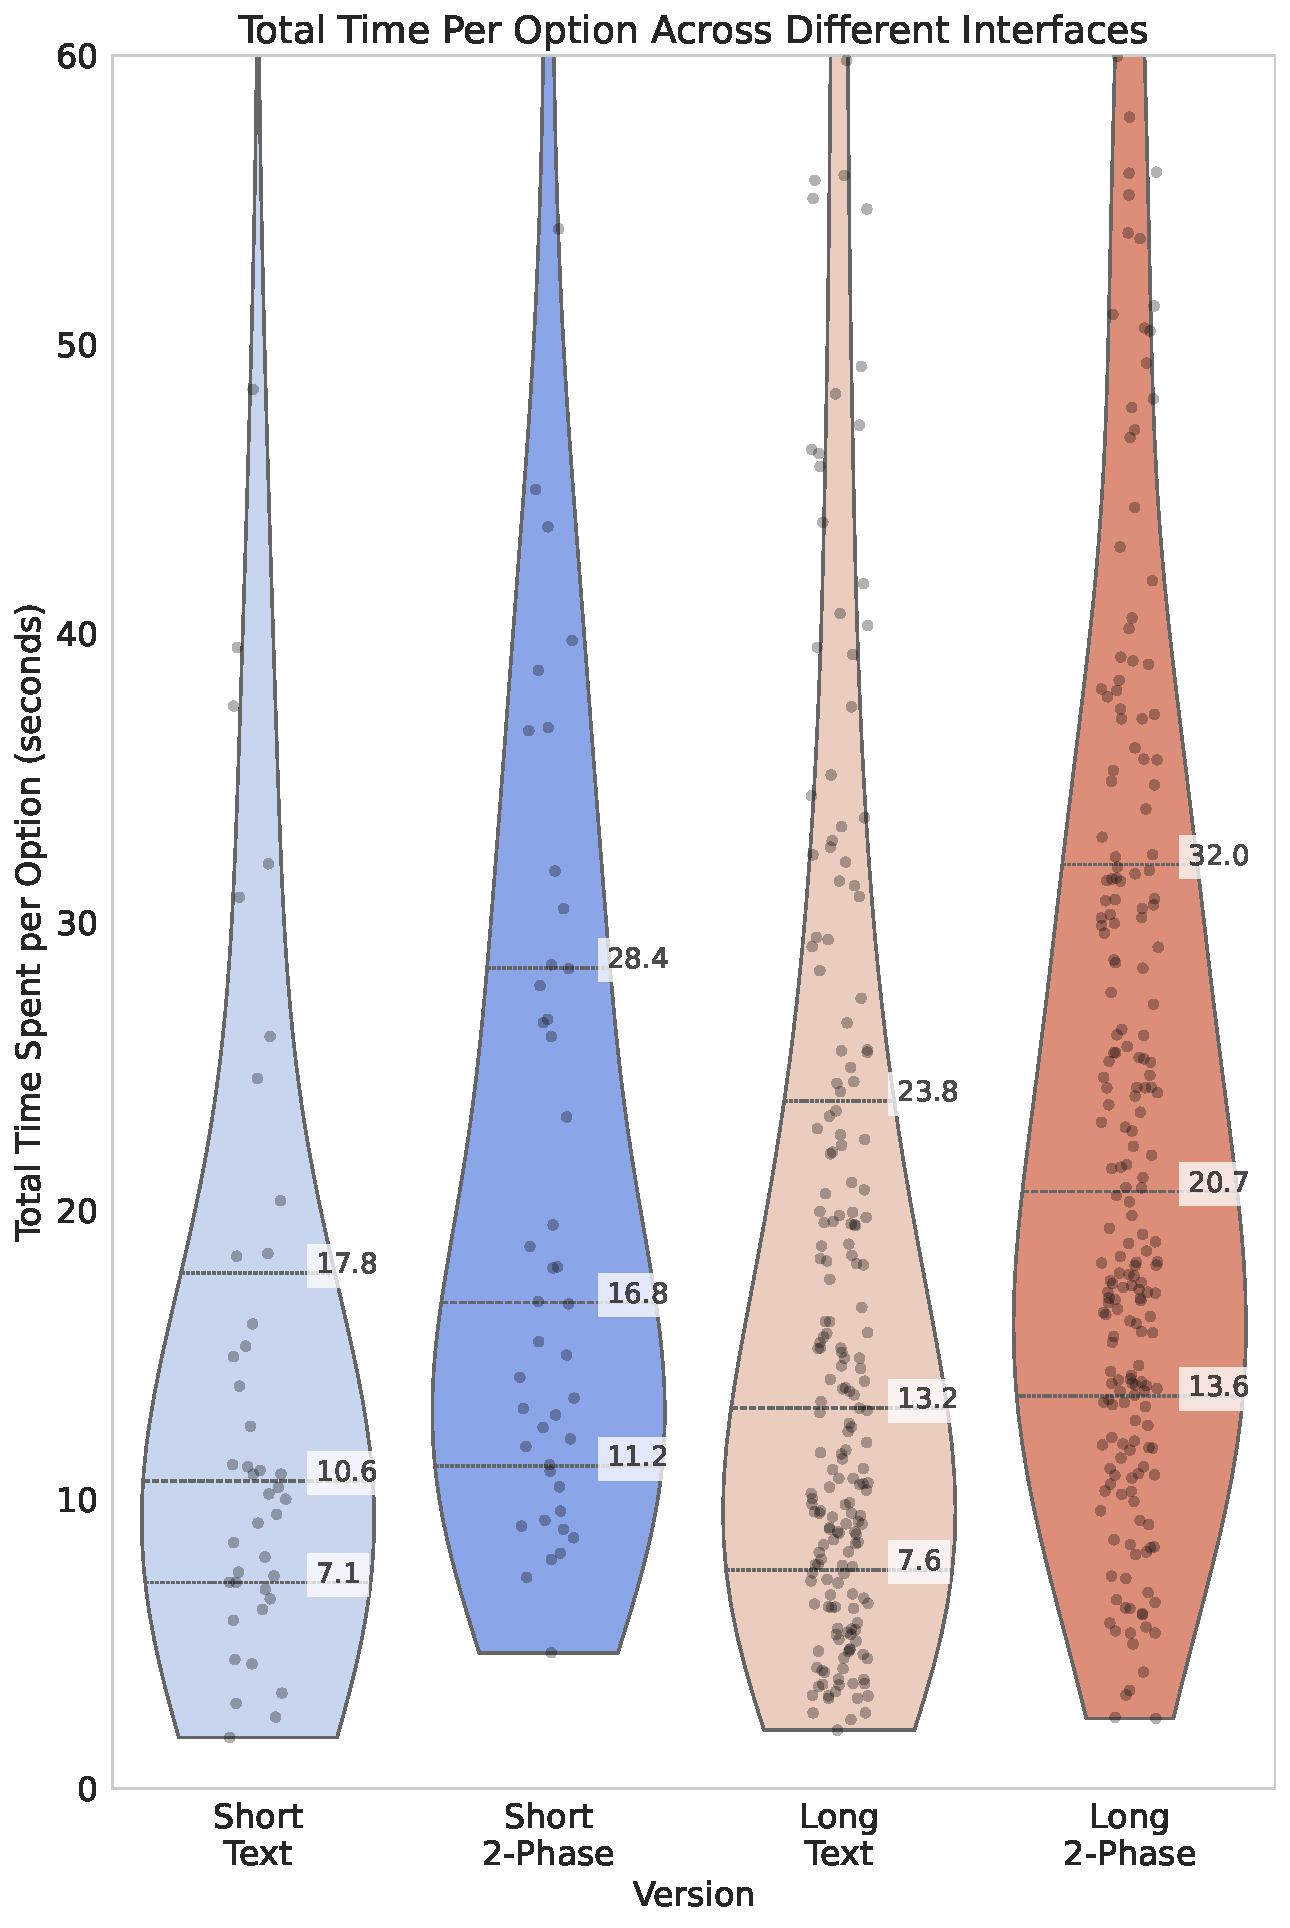
\includegraphics[width=0.95\textwidth, trim=0 10 0 10, clip]{content/image/results/total_time_per_option.pdf}
        \captionsetup{width=\textwidth, justification=justified} % Adjust the width to match the image width
        \caption{Total Time per option: We identified that the two-phase interface skewed slightly higher than the text interface, as expected. This discrepancy can be attributed to the extra organization step required in the two-phase interface, leading to a slightly longer overall completion time per option.}
        \Description{Violin plot showing total time spent per option in seconds across four interface versions: Short Text, Short 2-Phase, Long Text, and Long 2-Phase. The y-axis ranges from 0 to 60 seconds. Each violin plot has scattered dots representing individual data points. The shape of the Short Text plot is widest between 10 and 20 seconds, tapering at the top and bottom. The Short 2-Phase plot is the narrowest, with most dots concentrated between 10 and 20 seconds. The Long Text plot is narrow and widest near the bottom, between 5 and 15 seconds. The Long 2-Phase plot is widest near the top, between 20 and 40 seconds.}
        \label{fig:total_time}
    \end{subfigure}
    \hfill
    % Second subfigure
    \begin{subfigure}[b]{0.38\textwidth}
        \centering
        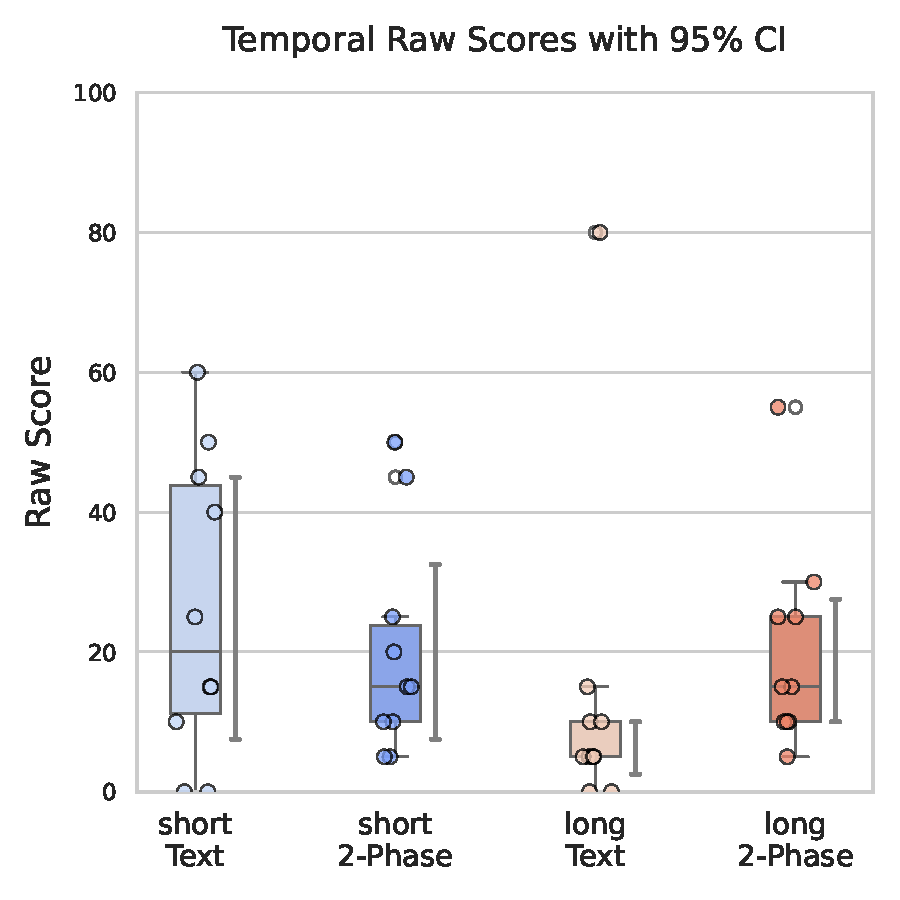
\includegraphics[width=0.95\textwidth, trim=0 13 0 13, clip]{content/image/cog/Temporal_scores.pdf}
        \captionsetup{width=\textwidth, justification=justified} % Adjust the width to match the image width
        \caption{Temporal Demand Raw Score: The short text interface results in the highest temporal demand, while the long text interface is the lowest. Two-phase interfaces show moderate temporal demand, suggesting that interactive elements allowed participants to pace themselves better.}
        \label{fig:temporal_cog_score}
    \end{subfigure}
\end{figure}

From the qualitative results regarding temporal demand, we find notable differences. While 37.5\% of participants (N=15) attributed time to \textit{Decision Making} as a source of temporal demand, they framed it differently. First, 50\% of participants (N=5) in the long two-phase group described the pressure to make decisions affirmatively. This suggests that their pressure stemmed from having too many remaining decisions to make~(\smallquote{S022}{So it didn't take too much time, but obviously there were a lot of things to consider, so there was some temporal demand.}) and not from the time they had already spent. This is reflective of the additional time spent by participants in the two-phase interface reflecting their active engagement but their pressure to complete the task in a timely manner. Conversely, in the short text group, 50\% of participants (N=5) expressed concern about the time and effort they had already invested~(\smallquote{S024}{maybe I should just hurry up and make a decision.}) and none framed it affirmatively. In other words, participants expected to complete the task sooner than they actually did. This response potentially explains why participants in the short text interface exhibited a higher trend in temporal demand (Fig.~\ref{fig:temporal_cog_score}, and Appendix X for Bayesian pairwise comparison) compared to the other experimental groups. 

Surprisingly, participants in the long text interface exhibited the lowest temporal demand (Figure~\ref{fig:temporal_cog_score}), despite spending more time per option and traversing the longest distance (Section~\ref{sec:dist}). Only 30\% of participants (N=3) mentioned the time spent making a decision as a source of temporal demand. One possible explanation is that some participants were satisficing, which we will discuss further in Section~\ref{ref:secsatisfice}.

\subsection{Budget and Voting Behaviors}
Resource allocation plays a significant role in influencing decision-making.\textcite{chengCanShowWhat2021} demonstrated that the number of credits allocated influences the validity of Quadratic Voting (QV). Decision science studies, such as \textcite{Shah2015a} and \cite{debruijnPovertyEconomicDecision2022}, have shown that scarcity influences decision-making, increases risk aversion, and adds cognitive load. These measures act as proxies for understanding participant behavior. We further break down and highlight key differences in how participants in long Quadratic Surveys (QS) adjusted their voting behaviors as credits changed, with a detailed analysis provided in Appendix~\ref{apdx:additional_results_behavior}.

\begin{figure}[h]
    \centering
    \begin{subfigure}[b]{\textwidth}
        \centering
        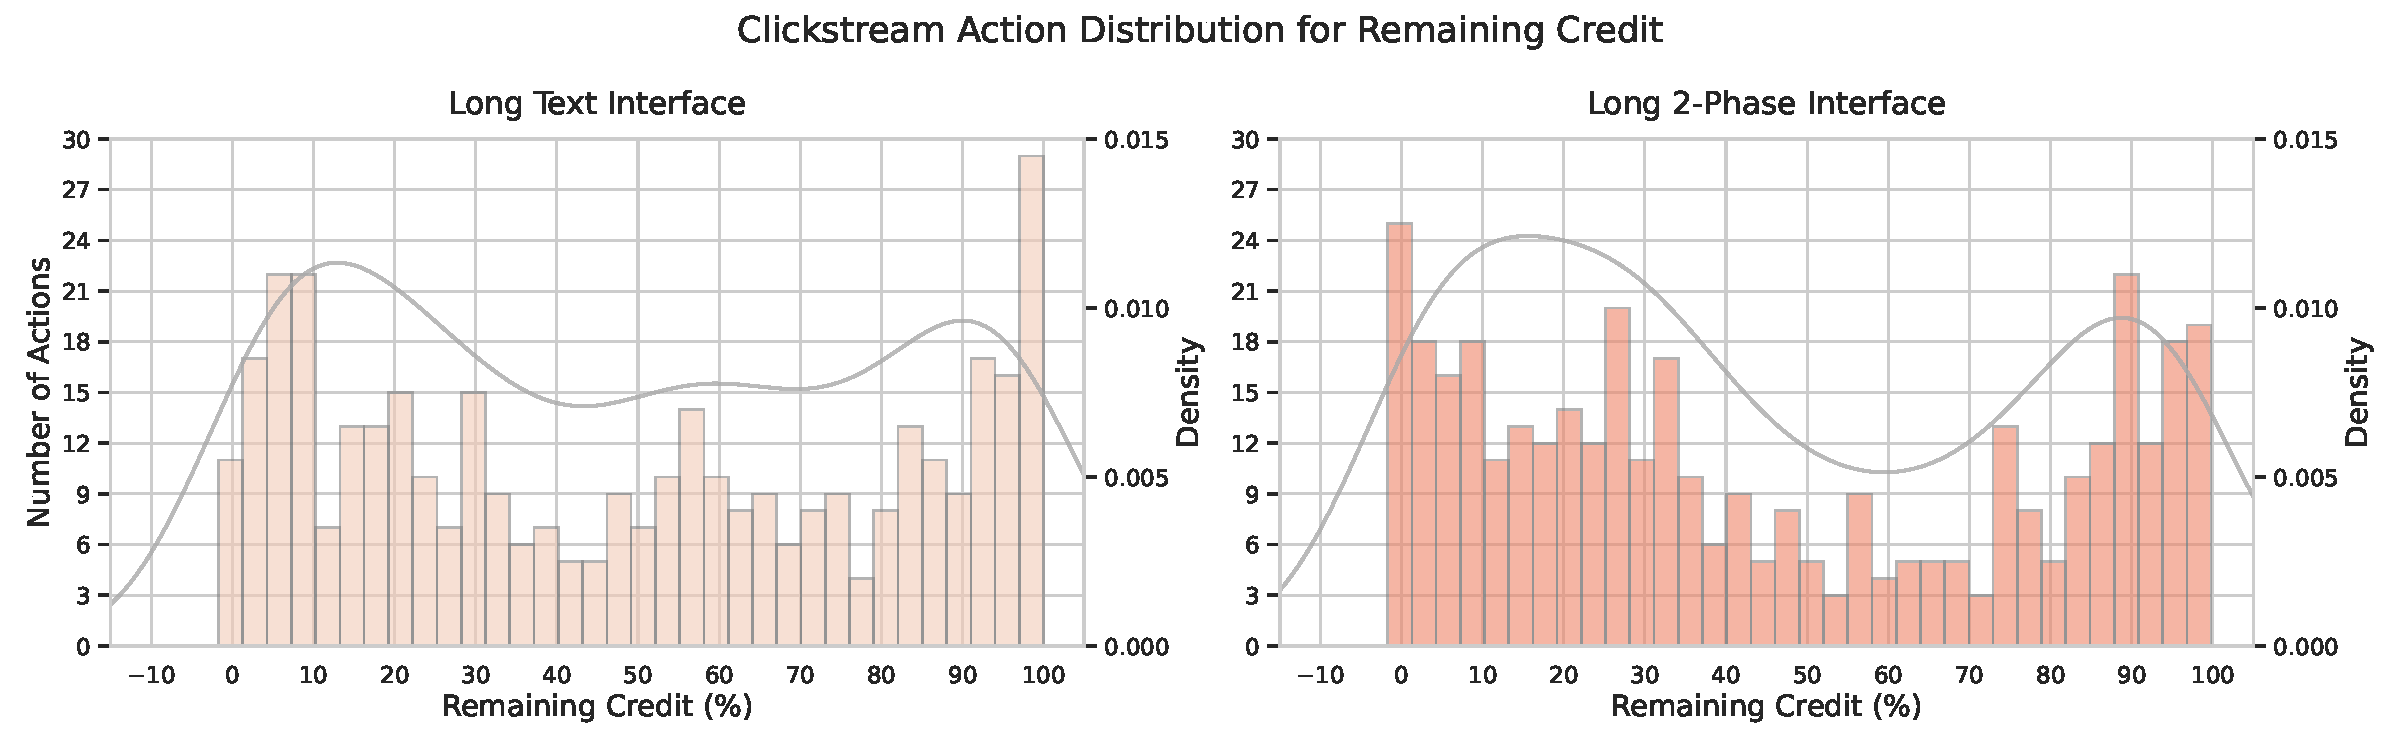
\includegraphics[width=\textwidth]{content/image/results/new_clickstream_action_distribution_lower_row.pdf}
        \caption{This plot counts the number of voting actions when there are $x$ percentages of credits remaining. A KDE plot is provided to help better understand the action distribution.}
        \Description{A dual-panel histogram with overlaid KDE curves showing the distribution of voting actions based on remaining credit percentages for two interfaces: Long Text and Long 2-Phase. The x-axis shows the remaining credit as a percentage, ranging from -10\% to 100\%, and the y-axis on the right shows density for the KDE curves. In the left panel for the Long Text interface, the KDE curve rises sharply to a peak around 10\%, gradually declines, and then rises again toward 100\%, with a moderate dip in the middle. In the right panel for the Long 2-Phase interface, the KDE curve shows more pronounced changes: it rises steadily from 10\% to 30\%, then dips more sharply than the left panel, before rising to a prominent peak near 100\%. The right curve has a deeper dip and a broader rise compared to the left.}
        \label{fig:all_clicks}
    \end{subfigure}
    
    \vspace{1em} % Adjusts the space between the subplots
    
    \begin{subfigure}[b]{\textwidth}
        \centering
        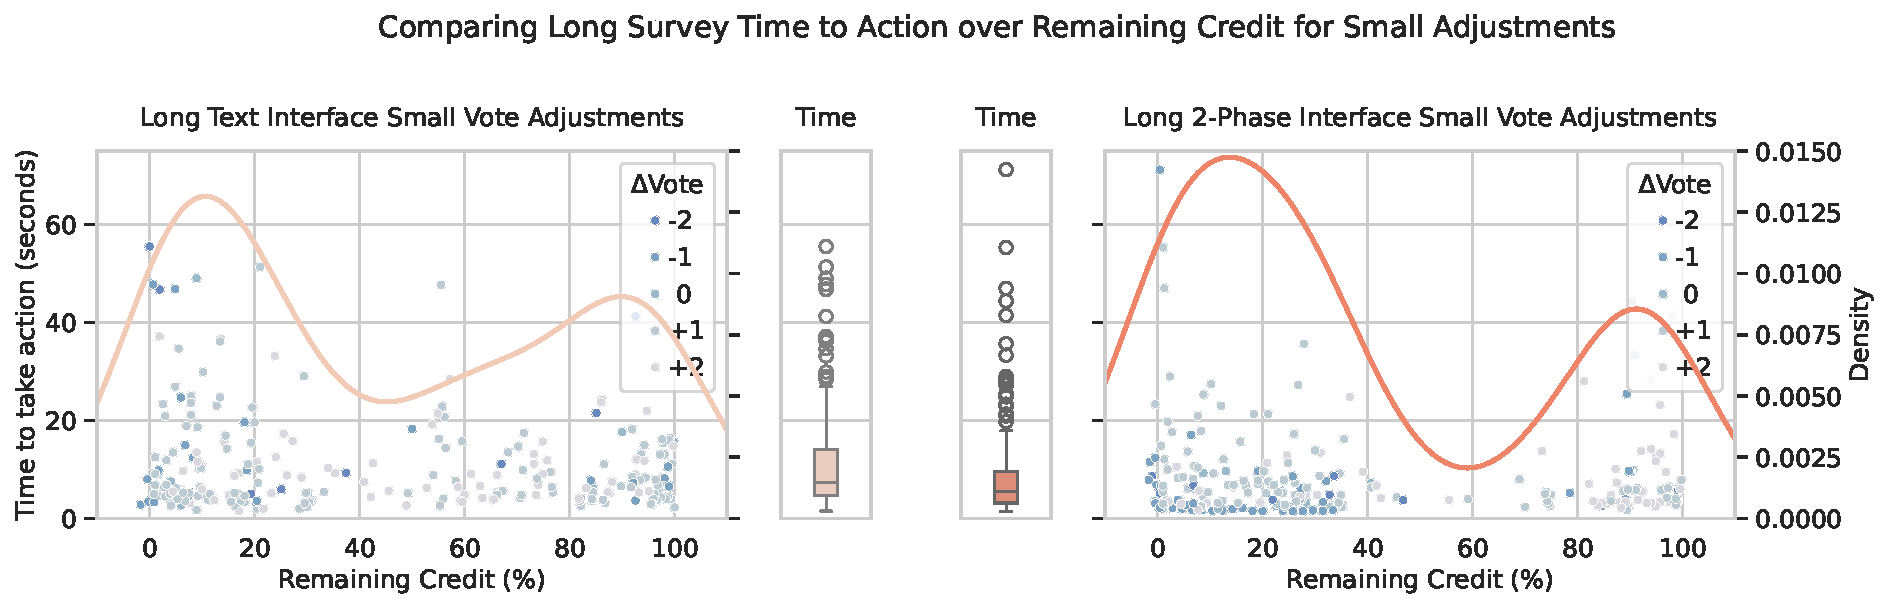
\includegraphics[width=\textwidth]{content/image/results/small_adjustments_plot.pdf}
        \caption{This plot further separates participants' interaction behavior based on the number of votes participants adjusted. We observed a bimodal interaction pattern across long QS when small vote adjustments are made.}
        \Description{A dual-panel plot comparing time to take action in seconds over remaining credit percentages for small vote adjustments in two interfaces: Long Text and Long 2-Phase. The x-axis shows remaining credit as a percentage, from 0\% to 100\%, and the y-axis on the left shows the time to take action in seconds, ranging from 0 to 60. Both panels feature scatter plots with colored dots representing vote changes from -2 to +2. The left panel shows the Long Text interface, with an orange density line rising sharply, peaking around 20\% remaining credit, then dipping around 50\%, and rising again near 100\%. The right panel shows the Long 2-Phase interface with a similar pattern, but the peaks and dips are more pronounced, especially with a sharper dip near 50\%. A box plot on the far right summarizes action time, showing the spread and median time for each interface.}

        \label{fig:small_clicks}
    \end{subfigure}
    
    \caption{Comparison of voting actions and participant behavior in different survey interfaces. Subplot (a) shows the overall distribution of actions based on the remaining credit, while subplot (b) further differentiates the interaction based on the size of vote adjustments.}
    \Description{This figure contains two subfigures stacked on top of one another.}
    \label{fig:combined_voting_behavior}
\end{figure}

Figure~\ref{fig:all_clicks} presents the number of vote adjustments made at a given remaining budget across the two interfaces. Figure~\ref{fig:small_clicks} visualizes vote adjustments of two or fewer votes, representing $10\%$ of the possible values participants could select from a maximum of 21 votes. A kernel density estimate (KDE) plot illustrates how these actions were distributed across the remaining credits. A higher density indicates more actions at a given percentage of remaining credits over all actions.

In long surveys, participants exhibited more voting actions both when their budgets were abundant and when they began to deplete. This pattern was more pronounced in the long two-phase interface, as evident from the higher KDE plots for small vote adjustments. When budgets fell below 50\%, The kernel density curve of the long two-phase interface position above that of the long text interface, along with the more visually clustered dots, indicates that participants in the long two-phase interface made more frequent and smaller adjustments. This suggests that participants in the two-phase interface remained engaged even when budgets were limited, potentially reflecting their effort to fine-tune vote allocations. This aligns with our qualitative findings, where 12.5\% of participants (N=5) highlighted how the interface supported their incremental and iterative approach during interviews; all of these participants used the two-phase interface.

\begin{displayquote}
I like the fact that it remembers everything that you know.~\bracketellipsis that's very important is that it's an iterative process.\hfill\quoteby{S019 (LI)}
\end{displayquote}



%%%%%%%%%%%%%%%%%%%%%%%%%%%%%%%%%%%%% Other useful text %%%%%%%%%%%%%%%%%%%%%%%%%%%%%%%%%%%%%%


% \subsection{Summary across all cognitive load dimensions}
% Overall, participants using the two-phase interface tended to think more comprehensively and critically, while those using the text interface focused more on operational tasks. This is reflected by~\textit{mental demand} findings where participants using the text interface reported greater difficulty in determining the precise number of votes. In contrast, participants using the long two-phase interface were more likely to consider broader societal impacts and evaluate options holistically.~\textit{Effort} echoes similar findings. In terms of~\textit{physical demand}, participants using the two-phase interface, particularly in longer surveys, experienced higher demand due to increased mouse usage, which was expected. Additionally, participants using the short text interface wanted to complete the task quickly and reported the highest ~\textit{temporal demand}, while those using the long text interface reported the lowest. Moreover, participants using the long text interface exhibited the least amount of~\textit{frustration} from operational causes compared to other experimental conditions. Thus, we suspect that participants who completed the long QS on a text interface engaged in satisficing behaviors, based on the counter-intuitive results showing they had the lowest temporal demand and frustration levels. Finally, in relation to~\textit{performance}, participants using the two-phase interface more frequently reported positive feelings about their final submissions, suggesting greater confidence in their decision-making process. We will interpret these results in the discussion section. To better understand participants' behavior, we analyze click-stream data across experimental conditions in the next section.

%%%%%%%%%%%%%%%%%%%%%%%%%%%%%%%%%%%%%% Satisficing evidence %%%%%%%%%%%%%%%%%%%%%%%%%%%%%%%%%%%%%%
%$15$ participants highlighted this source for frustration. $6$ participants expressed frustration regarding credit management~(i.e., overspending budget); $4$ participants mentioned had trouble deciding the final value for the options; $3$ participants are frustrated because they need to make multiple decisions; $5$ participants were frustrated with the quadratic mechanism; $4$ participants are frustrated trying to understand the content of the option or how the option connects to them. For example, 

%\begin{displayquote}
%I was slightly frustrated when doing the task, probably because there was a budget that we kind of had to stick with it.

%\noindent \hfill -- S001, long text interface, quadratic mechanism
%\end{displayquote}

%\begin{displayquote}
%i think just frustration~\bracketellipsis because when i was making like the decisions on how many upvotes I could put in each section, I was running out of credits.

%\noindent \hfill -- S013, short two-phase interface, budget management
%\end{displayquote}